\documentclass[a4paper]{report}

% text
\usepackage[utf8]{inputenc}
\usepackage[numbers]{natbib}
%\bibliographystyle{unsrtnat}
\usepackage{lipsum}
\usepackage[toc,page]{appendix}
\usepackage{amssymb,amsmath}
\usepackage{gensymb}
\usepackage{amsfonts}
\usepackage{todonotes}
\usepackage{listings}
\usepackage{enumitem}
\usepackage{scrextend}
\usepackage{graphicx, xcolor}
\usepackage{wrapfig}
\usepackage{rotating}
\usepackage{subcaption, float}
\usepackage{titlesec}
\usepackage{verbatim}
\usepackage[document]{ragged2e} % Right and left aligned text
%\usepackage[sc]{titlesec}
%\usepackage{titletoc}

% links
\usepackage{color}
%\usepackage[linktocpage=true, colorlinks=true, allcolors=blue]{hyperref}
\usepackage[pdfpagemode={UseOutlines},bookmarks=true,bookmarksopenlevel=0,bookmarksnumbered=true,plainpages=false,colorlinks,linkcolor={black},citecolor={blue},urlcolor={blue},pdfstartview={FitV},unicode,breaklinks=true,pdfpagelabels]{hyperref}
\usepackage[all]{hypcap}
\usepackage[hypcap]{caption}

% layout
%\usepackage{multicol}
\usepackage{fancyhdr,lastpage}
\setcounter{tocdepth}{2}

% header layout
\usepackage{suffix}

% Abbreviations and glossary
\usepackage[automake,entrycounter,acronym,toc,section=section,numberedsection=autolabel]{glossaries-extra}
\makeglossaries\setabbreviationstyle[acronym]{long-postshort-user}
\glssetcategoryattribute{acronym}{nohyperfirst}{true}
\renewcommand*{\glsxtruserparen}[2]{
  \glsxtrfullsep{#2}
  (\glshyperlink[#1]{#2})
}

%% Name of the project, can always be called by: \project
\newcommand{\project}{\emph{VHF-Unit}}	

%% Pictures with aurthor and source
\newcommand\chapterauthor[1]{\authortoc{#1}\printchapterauthor{#1}}
\WithSuffix\newcommand\chapterauthor*[1]{\printchapterauthor{#1}}

\makeatletter
\newcommand{\printchapterauthor}[1]{%
  {\parindent0pt\vspace*{-10pt}%
  \linespread{1.1}\large\scshape#1%
  \par\nobreak\vspace*{10pt}}
  \@afterheading%
}
\newcommand{\authortoc}[1]{%
  \addtocontents{toc}{\vskip-1pt}%
  \addtocontents{toc}{%
    \protect\contentsline{chapter}%
    {\hskip0em\mdseries\scshape\protect\scriptsize#1}{}{}}
  \addtocontents{toc}{\vskip5pt}%
}
\makeatother


%% Fixed 4th deepth
%\setcounter{secnumdepth}{4}
%\titleformat{\paragraph}
%{\normalfont\normalsize\bfseries}{\theparagraph}{1em}{}
%\titlespacing*{\paragraph}
%{0pt}{1.25ex plus 1ex minus .2ex}{0.5ex plus .2ex}

% Chapter and section style
\titleformat
{\chapter} % command
[display] % shape
{\bfseries\huge} % format
{ \ \thechapter} % label
{0.5ex} % sep
{
    \rule{\textwidth}{1pt}
    \vspace{0ex}
    \centering
} % before-code


%\titleformat{\section}[wrap]
%{\Large\bfseries}
%{\thesection}{0.5em}{}
%\titlespacing{\section}{10pc}{1.5ex plus .1ex minus .2ex}{1pc}
 


% Figure caption source
\newcommand*{\captionsource}[2]{%
  \caption[{#1}]{#1}\par
  \textbf{Source:} #2\par}

% header style
\pagestyle{fancy}
\lhead{Project \project}
\chead{}

\rhead{\today}
\lfoot{}
\cfoot{\thepage~of~\pageref{LastPage}}
\rfoot{}
\renewcommand{\headrulewidth}{0.4pt}
\renewcommand{\footrulewidth}{0.4pt}

%%% API
%%% The glossary entry the acronym links to   

\begin{comment}

\newglossaryentry{apig}{name={API},
    description={An Application Programming Interface (API) is a particular set
    of rules and specifications that a software program can follow to access and
    make use of the services and resources provided by another particular software
    program that implements that API. }}

%%% define the acronym and use the see= option
\newglossaryentry{api}{type=\acronymtype, name={API}, 
description={Application Programming Interface}, 
first={Application Programming Interface (API)\glsadd{apig}}, see=[Glossary:]{apig}}

%%% TOF
\newglossaryentry{tofg}{name={ToF},
    description={Time of Flight (TOF) is a property of an object, particle, electromagnetic or other wave. It is the time that such an object needs to travel a distance through a medium. The measurement of this time (i.e. the time of flight) can be used for a time standard as a way to measure velocity or path length through a given medium.}}
\newglossaryentry{tof}{type=\acronymtype, name={ToF}, 
description={Time of Flight}, 
first={Time of Flight (TOF)\glsadd{tofg}}, see=[Glossary:]{tofg}}
\end{comment}

%%% ti
\newglossaryentry{tig}{name={TI},
    description={Texas Instruments Inc. (TI) is an American technology company
	that designs and manufactures semiconductors and various integrated circuits. }}
\newglossaryentry{ti}{type=\acronymtype, name={TI}, 
description={Texas Instruments Inc.}, 
first={Texas Instruments Inc. (TI)\glsadd{tig}}, see=[Glossary:]{tig}}

%%% IC
\newglossaryentry{icg}{name={IC},
    description={Integrated Circuit (IC) is a set of electronic circuits on one small flat chip.}}
\newglossaryentry{ic}{type=\acronymtype, name={IC}, 
description={Integrated Circuit}, 
first={Integrated Circuit (IC)\glsadd{icg}}, see=[Glossary:]{icg}}

%%% PC
\newglossaryentry{pcg}{name={PC},
    description={Personal Computer (PC)  is a multi-purpose computer whose size,
	capabilities, and price make it feasible for individual use.}}
\newglossaryentry{pc}{type=\acronymtype, name={NAME}, 
description={Personal Computer}, 
first={Personal Computer (PC)\glsadd{pcg}}, see=[Glossary:]{pcg}}

%%% IMU
\newglossaryentry{imug}{name={IMU},
    description={Inertial Measurement Units (IMUs) are integrated circuits that
    can measure acceleration, rotational velocity and magnetic field strength.}}
\newglossaryentry{imu}{type=\acronymtype, name={IMU}, 
description={Inertial Measurement Unit}, 
first={Inertial Measurement Unit (IMU)\glsadd{imug}}, see=[Glossary:]{imug}}

%%% LDO
\newglossaryentry{ldog}{name={LDO},
    description={A low-dropout regulator is a DC linear voltage regulator that can regulate the output voltage even when the supply voltage is very close to the output voltage.}}
\newglossaryentry{ldo}{type=\acronymtype, name={LDO}, 
description={Low-dropout regulator}, 
first={Low-dropout regulator (LDO)\glsadd{ldog}}, see=[Glossary:]{ldog}}

%%% RTC
\newglossaryentry{rtcg}{name={RTC},
    description={A Real time clock is an IC that is used to mesure time even when the main device is off.}}
\newglossaryentry{rtc}{type=\acronymtype, name={RTC}, 
description={Real time clock}, 
first={Real time clock (RTC)\glsadd{rtcg}}, see=[Glossary:]{rtcg}}

%%% JTAG
\newglossaryentry{jtagg}{name={JTAG},
    description={JTAG is an industry standard for verifying designs and testing printed circuit boards after manufacture.}}
\newglossaryentry{jtag}{type=\acronymtype, name={JTAG}, 
description={Joint Test Action Group}, 
first={Joint Test Action Group (JTAG)\glsadd{jtagg}}, see=[Glossary:]{jtagg}}

%%% GPS
\newglossaryentry{gpsg}{name={GPS},
    description={The Global Positioning System (GPS) is a radionavigation
    system owned by the United States government and operated by the 
    United States Air Force. It uses sattelites for geolocation and time.}}
\newglossaryentry{gps}{type=\acronymtype, name={GPS}, 
description={Global Positioning System}, 
first={Global Positioning System (GPS)\glsadd{gpsg}}, see=[Glossary:]{gpsg}}

%%% CAD
\newglossaryentry{cadg}{name={CAD},
    description={Computer-aided design (CAD) is a computer system which aids
    the creation and modification of some kind of design.}}
\newglossaryentry{cad}{type=\acronymtype, name={CAD}, 
description={Computer-aided design}, 
first={Computer-aided design (CAD)\glsadd{cadg}}, see=[Glossary:]{cadg}}

%%% MCU
\newglossaryentry{mcug}{name={MCU},
    description={A Microcontroller Unit (MCU) is a single computer chip 
    designed for embedded applications.}}
\newglossaryentry{mcu}{type=\acronymtype, name={MCU}, 
description={Microcontroller Unit}, 
first={Microcontroller Unit (MCU)\glsadd{mcug}}, see=[Glossary:]{mcug}}

%%% PCB
\newglossaryentry{pcbg}{name={PCB},
    description={A Printed Circuit Board (PCB) is the common acronym when
	referring to populated circuit boards.}}
\newglossaryentry{pcb}{type=\acronymtype, name={PCB}, 
description={Printed Circuit Board}, 
first={Printed Circuit Board (PCB)\glsadd{pcbg}}, see=[Glossary:]{pcbg}}

%%% PWB
\newglossaryentry{pwbg}{name={PWB},
    description={A Printed Wire Board (PWB) is the common acronym when
	referring to unpopulated circuit boards.}}
\newglossaryentry{pwb}{type=\acronymtype, name={PWB}, 
description={Printed Wire Board}, 
first={Printed Wire Board (PWB)\glsadd{pwbg}}, see=[Glossary:]{pwbg}}

%\begin{comment}
%%% SEK
\newglossaryentry{sekg}{name={SEK},
    description={Swedish Krona (SEK) is the currency in Sweden.}}
\newglossaryentry{sek}{type=\acronymtype, name={SEK}, 
description={Swedish Krona}, 
first={Swedish Krona (SEK)\glsadd{sekg}}, see=[Glossary:]{sekg}}

%%% SWD
\newglossaryentry{swdg}{name={SWD},
    description={Serial Wire Debug (SWD) is an alternative 2-pin electrical interface,
	standard debugging protocol used in ARM processors.}}
\newglossaryentry{swd}{type=\acronymtype, name={SWD},
description={Serial Wire Debug}, 
first={Serial Wire Debug (SWD)\glsadd{swdg}}, see=[Glossary:]{swdg}}

%%% LI-ION
\newglossaryentry{liong}{name={LIB},
    description={Lithium-ion Battery (LIB) is a common type of rechargeable battery.}}
\newglossaryentry{lion}{type=\acronymtype, name={LIB}, 
description={Battery Management System}, 
first={Lithium-ion Batteries (LIB)\glsadd{liong}}, see=[Glossary:]{liong}}

%%% PTC 
\newglossaryentry{ptcg}{name={PTC},
	description={Positive Temperature Coefficient (PTC) describes the
	relative change of a physical property that is associated with a given change in temperature.}}
\newglossaryentry{ptc}{type=\acronymtype, name={PTC},
description={Positive Temperature Coefficient},
first={Positive Temperature Coefficient (PTC)\glsadd{ptcg}}, see=[Glossary:]{ptcg}}

%%% ST
\newglossaryentry{stg}{name={ST},
    description={STMicroelectronics (ST) is a French-Italian multinational 
    electronics and semiconductor manufacturer.}}
\newglossaryentry{st}{type=\acronymtype, name={ST}, 
description={STMicroelectronics}, 
first={STMicroelectronics (ST)\glsadd{stg}}, see=[Glossary:]{stg}}

%%% DRC
\newglossaryentry{drcg}{name={DRC},
    description={Design Rule Check (DRC) is an automated check of your designed \gls{pcb}
	to see if it follows all specified design rules.}}
\newglossaryentry{drc}{type=\acronymtype, name={DRC}, 
description={Design Rule Check}, 
first={Design Rule Check (DRC)\glsadd{drcg}}, see=[Glossary:]{drcg}}

%%% ERC
\newglossaryentry{ercg}{name={ERC},
    description={Electronic Rule Check (ERC) is an automated check of your designed schematic
	to see if it follows all electronic rules.}}
\newglossaryentry{erc}{type=\acronymtype, name={ERC}, 
description={Electronic Rule Check}, 
first={Electronic Rule Check (ERC)\glsadd{ercg}}, see=[Glossary:]{ercg}}

%%% USB
\newglossaryentry{usbg}{name={USB},
    description={Universal Serial Bus (USB), is an industry standard for
    cables, connectors and communications protocols for connection, 
    communication, and power supply between computers and devices.}}
\newglossaryentry{usb}{type=\acronymtype, name={USB}, 
description={Universal Serial Bus}, 
first={Universal Serial Bus (USB)\glsadd{usbg}}, see=[Glossary:]{usbg}}

%%% LED
\newglossaryentry{ledg}{name={LED},
    description={A Light-emitting diode (LED), is a two-lead semiconductor light source.}}
\newglossaryentry{led}{type=\acronymtype, name={LED}, 
description={Light-emitting diode}, 
first={Light-emitting diode (LED)\glsadd{ledg}}, see=[Glossary:]{ledg}}

%%% GPIO
\newglossaryentry{gpiog}{name={GPIO},
    description={General Purpose Input Output (GPIO), is a general use port of an \gls{mcu}.}}
\newglossaryentry{gpio}{type=\acronymtype, name={GPIO}, 
description={General Purpose Input Output}, 
first={General Purpose Input Output (GPIO)\glsadd{gpiog}}, see=[Glossary:]{gpiog}}

%%% SPI
\newglossaryentry{spig}{name={SPI},
    description={Serial Peripheral Interface Bus (SPI), is a synchronous 
    serial communication interface specification used for short distance 
    communication, primarily in embedded systems.}}
\newglossaryentry{spi}{type=\acronymtype, name={SPI}, 
description={Serial Peripheral Interface}, 
first={Serial Peripheral Interface (SPI)\glsadd{spig}}, see=[Glossary:]{spig}}

%%% I2C
\newglossaryentry{i2cg}{name={I$^2$C},
    description={Inter-Integrated Circuit (I$^2$C), is a serial computer bus.}}
\newglossaryentry{i2c}{type=\acronymtype, name={I$^2$C}, 
description={Inter-Integrated Circuit}, 
first={Inter-Integrated Circuit (I$^2$C)\glsadd{i2cg}}, see=[Glossary:]{i2cg}}

%%% ADC
\newglossaryentry{adcg}{name={ADC},
    description={An Analog-to-digital converter (ADC) is a system that converts 
    an analog signal into a digital signal.}}
\newglossaryentry{adc}{type=\acronymtype, name={ADC}, 
description={Analog-to-digital converter}, 
first={Analog-to-digital converter (ADC)\glsadd{adcg}}, see=[Glossary:]{adcg}}

%%% NMEA
\newglossaryentry{nmeag}{name={NMEA},
    description={The National Marine Electronics Association (NMEA) standard is a
    specification that defines the interface between various pieces of marine electronic equipment.}}
\newglossaryentry{nmea}{type=\acronymtype, name={NMEA}, 
description={National Marine Electronics Association standard}, 
first={National Marine Electronics Association standard (NMEA)\glsadd{nmeag}}, see=[Glossary:]{nmeag}}

%%% VIA
\newglossaryentry{viag}{name={VIA},
    description={A vertical interconnect access (via) is an electrical connection between
	layers in a physical electronic circuit.}}
\newglossaryentry{via}{type=\acronymtype, name={via}, 
description={vertical interconnect access}, 
first={via\glsadd{viag}}, see=[Glossary:]{viag}}

%%% PNG
\newglossaryentry{pngg}{name={PNG},
    description={Portable Network Graphics (PNG) is a raster graphics file format.}}
\newglossaryentry{png}{type=\acronymtype, name={PNG}, 
description={Portable Network Graphics}, 
first={Portable Network Graphics (PNG)\glsadd{pngg}}, see=[Glossary:]{pngg}}


%%% LGA
\newglossaryentry{lgag}{name={LGA},
    description={Land Grid Array (LGA) is a type of \gls{smd} device with pins on the socket.}}
\newglossaryentry{lga}{type=\acronymtype, name={LGA}, 
description={Land Grid Array}, 
first={Land Grid Array (LGA)\glsadd{lgag}}, see=[Glossary:]{lgag}}

%%% SMD
\newglossaryentry{smdg}{name={SMD},
    description={Surface Mount Devices (SMD) are electric components soldered directly on a \gls{pcb} instead of using through-holes.}}
\newglossaryentry{smd}{type=\acronymtype, name={SMD}, 
description={Surface Mount Device}, 
first={Surface Mount Device (SMD)\glsadd{smdg}}, see=[Glossary:]{smdg}}

%%% IPC
\newglossaryentry{ipcg}{name={IPC},
    description={Institute for Printed Circuits (IPC), Institute for Interconnecting and Packaging Electronic Circuits}}
\newglossaryentry{ipc}{type=\acronymtype, name={IPC}, 
description={Institute for Printed Circuits}, 
first={Institute for Printed Circuits (IPC)\glsadd{ipcg}}, see=[Glossary:]{ipcg}}


%\end{comment}
\thispagestyle{empty}



\begin{document}

\begin{titlepage}
\newcommand{\HRule}{\rule{\linewidth}{0.5mm}}
\center % Centre everything on the page

%------------------------------------------------
%	Headings
%------------------------------------------------

\textsc{\LARGE Luleå University of Technology}\\[1.5cm] % Main heading such as the name of your university/college

\textsc{\Large Dept.\ of Computer Science, Electrical and Space Engineering}\\[0.5cm] % Major heading such as course name

\begin{centering}
\begin{tabular}{l l}
\textsc{\large X7005E --}	& \textsc{\large Master Thesis Engineering Physics and Electrical Engineering}\\ % Minor heading such as course title
				& \textsc{\large Electrical engineering} % Minor heading such as course title
\end{tabular}
\end{centering}\\[0.5cm]
%------------------------------------------------
%	Title
%------------------------------------------------

\HRule\\[0.8cm]

{\huge\bfseries Master Thesis Engineering Physics and Electrical Engineering \project}\\[0.4cm] % Title of your document

\HRule\\[1.5cm]

%------------------------------------------------
%	Author(s)
%------------------------------------------------
\begin{minipage}{0.4\textwidth}
	\begin{flushleft}
		\large
		\emph{Author}\\
		Lundberg, Josef, \\ 
	\end{flushleft}
\end{minipage}
~
\begin{minipage}{0.4\textwidth}
	\begin{flushright}
		\large
		\textit{Supervisor at the company}\\
		Evertsson, Bengt
	\end{flushright}
	\begin{flushright}
		\large
		\textit{Supervisor at the university}\\
		van Deventer, Jan?
	\end{flushright}
\end{minipage}

% If you don't want a supervisor, uncomment the two lines below and comment the code above
%{\large\textit{Author}}\\
%John \textsc{Smith} % Your name

%------------------------------------------------
%	Date
%------------------------------------------------

\vfill\vfill\vfill % Position the date 3/4 down the remaining page

{\large\today} % Date, change the \today to a set date if you want to be precise

%------------------------------------------------
%	Logo
%------------------------------------------------

\vfill\vfill

\includegraphics[width=0.2\textwidth]{Figures/ltu.jpg}\\[2cm] % Include a department/university logo - this will require the graphicx package
 
%----------------------------------------------------------------------------------------
\thispagestyle{empty}
\vfill % Push the date up 1/4 of the remaining page


\end{titlepage}

\clearpage
%\begin{abstract}
\chapter*{Abstract}



Surveillance and control has come a long way the last years. Every new mobile phone, most cars and smart watches have a GPS tracing device built in to it. Today it is hard to go anywhere without there beeing some sort of way of finding you. The art of finding has been around for a long time and one company that have taken the tracking aspect to the next step is Followit. For over 40 years they have built different types of GPS and radio transmitters to keep track of everything from small animals like hares and dogs to big elephants. They also got tracking solutions for vehicles like trucks and excavators. 


\thispagestyle{empty}
%\end{abstract}

% Preface
\clearpage
\chapter*{Preface}
\vspace{-10ex}%
\rule{\textwidth}{0.3pt}
\vspace{5ex}
 % after-code


I would like to thank the personal at Followit to taking me in and helping me through the project time. A special thanks to Bengt Evertsson for his supervision and help. 

A big thanks goes to my supervisor Jonny Johansson at LTU for his support and guidance in the project.
And a big thanks goes to my lovley fiancee Sara Andersson for her support and strong patience throughout the whole project. 

\begin{flushright}
Josef Lundberg
\newline
Lindesberg, \today
\end{flushright}

\begin{comment}
- Rätta till bilden med VHF skalan
- Räkna och visa den koplexa polerna mm för chebychev


\newglossaryentry{apig}{name={API},
    description={An Application Programming Interface (API) is a particular set
    of rules and specifications that a software program can follow to access and
    make use of the services and resources provided by another particular software
    program that implements that API. }}
%%% SWD
\newglossaryentry{swdg}{name={SWD},
    description={Serial Wire Debug (SWD) is an alternative 2-pin electrical interface,
	standard debugging protocol used in ARM processors.}}

\newglossaryentry{swd}{type=\acronymtype, name={SWD},
description={Serial Wire Debug}, 
first={Serial Wire Debug (SWD)\glsadd{swdg}}}
%%% define the acronym and use the see= option
\newglossaryentry{api}{type=\acronymtype, name={API}, 
description={Application Programming Interface}, 
first={Application Programming Interface (API)\glsadd{apig}}, see=[Glossary:]{apig}}
%%% TOF
\newglossaryentry{tofg}{name={ToF},
    description={Time of Flight (TOF) is a property of an object, particle, electromagnetic or other wave. It is the time that such an object needs to travel a distance through a medium. The measurement of this time (i.e. the time of flight) can be used for a time standard as a way to measure velocity or path length through a given medium.}}
\newglossaryentry{tof}{type=\acronymtype, name={ToF}, 
description={Time of Flight}, 
first={Time of Flight (TOF)\glsadd{tofg}}, see=[Glossary:]{tofg}}
%%% NMEA
\newglossaryentry{nmeag}{name={NMEA},
    description={The National Marine Electronics Association (NMEA) standard is a
    specification that defines the interface between various pieces of marine electronic equipment.}}
\newglossaryentry{nmea}{type=\acronymtype, name={NMEA}, 
description={National Marine Electronics Association standard}, 
first={National Marine Electronics Association standard (NMEA)\glsadd{nmeag}}}


%%% PNG
\newglossaryentry{pngg}{name={PNG},
description={ddddddddddddddddddddddddddddd}}

\newglossaryentry{png}{type=\acronymtype, name={PNG}, 
description={Portable Network Graphics (PNG) is a raster graphics file format.}, 
first={Portable Network Graphics (PNG)\glsadd{pngg}}}



%%% LED
\newglossaryentry{ledg}{name={LED},
description={sdf}}

\newglossaryentry{led}{type=\acronymtype, name={LED}, 
description={A Light-emitting diode (LED), is a two-lead semiconductor light source.}, 
first={Light-emitting diode (LED)\glsadd{ledg}}}


%%% LI-ION
\newglossaryentry{liong}{name={LIB},
    description={Lithium-ion Battery (LIB) is a common type of rechargeable battery.}}

\newglossaryentry{lion}{type=\acronymtype, name={LIB}, 
description={Battery Management System}, 
first={Lithium-ion Batteries (LIB)\glsadd{liong}}}


%%% PTC 
\newglossaryentry{ptcg}{name={PTC},
description={dddddddddddddddddddddddddddddddddddddddddddd}}

\newglossaryentry{ptc}{type=\acronymtype, name={PTC},
description={Positive Temperature Coefficient (PTC) describes the
	relative change of a physical property that is associated with a given change in temperature.},
first={Positive Temperature Coefficient (PTC)\glsadd{ptcg}}}


%%% PWB
\newglossaryentry{pwbg}{name={PWB},
description={ddddddddddddddddddddddddddddddddddd}}

\newglossaryentry{pwb}{type=\acronymtype, name={PWB}, 
description={A Printed Wire Board (PWB) is the common acronym when
	referring to unpopulated circuit boards.}, 
first={Printed Wire Board (PWB)\glsadd{pwbg}}}


%%% SEK
\newglossaryentry{sekg}{name={SEK},
description={werwerwer}}

\newglossaryentry{sek}{type=\acronymtype, name={SEK}, 
description={Swedish Krona (SEK) is the currency in Sweden.}, 
first={Swedish Krona (SEK)\glsadd{sekg}}}


%%% SMD
\newglossaryentry{smdg}{name={SMD},
description={rwerwer}}

\newglossaryentry{smd}{type=\acronymtype, name={SMD}, 
description={Surface Mount Devices (SMD) are electric components soldered directly on a \gls{pcb} instead of using through-holes.}, 
first={Surface Mount Device (SMD)\glsadd{smdg}}}


%%% ST
\newglossaryentry{stg}{name={ST},
description={ffffffffffffffffffffffff}}

\newglossaryentry{st}{type=\acronymtype, name={ST}, 
description={STMicroelectronics (ST) is a French-Italian multinational 
    electronics and semiconductor manufacturer.}, 
first={STMicroelectronics (ST)\glsadd{stg}}}


%%% TI
\newglossaryentry{tig}{name={TI},
description={ dddddddddddddddddddddddddddddd}}

\newglossaryentry{ti}{type=\acronymtype, name={TI}, 
description={Texas Instruments Inc. (TI) is an American technology company
	that designs and manufactures semiconductors and various integrated circuits.}, 
first={Texas Instruments Inc. (TI)\glsadd{tig}}}


%%% USB
\newglossaryentry{usbg}{name={USB},
description={ssddddddddddddddddddddddddddddddddddddddddddddd}}

\newglossaryentry{usb}{type=\acronymtype, name={USB}, 
description={Universal Serial Bus (USB), is an industry standard for
    cables, connectors and communications protocols for connection, 
    communication, and power supply between computers and devices.}, 
first={Universal Serial Bus (USB)\glsadd{usbg}}}


%%% VIA
\newglossaryentry{viag}{name={VIA},
description={dddddddddddddddddddddddddddddddddddddddddddddddddddddddddddd}}

\newglossaryentry{via}{type=\acronymtype, name={VIA}, 
description={A vertical interconnect access (via) is an electrical connection between
	layers in a physical electronic circuit.}, 
first={Vertical Interconnect Access\glsadd{viag}}}




\end{comment}

%\thispagestyle{empty}

\clearpage
\setlength{\columnseprule}{0.2pt}
\tableofcontents % TABLE OF CONTENTS
\vspace{0.5em}

\clearpage

%\setlength{\parindent}{0pt}
\printglossary[type=\acronymtype]
\noindent
\printglossary[type=main]

\clearpage
\setcounter{page}{2}
\chapter{Introduction}

This is not a new area of pruducts for Followit, they have made radio sending units for over 40? years.
When new and improved technology arrives every yerar you need to make new products to have the latest most efficiant and effective systems. Every generation of a komponent will most likley have a smaller physical size, have more advanced features and draw less power The wants to make a new unit 
Customers have been asking for a simple, small and cheap radio unit from the company to complemet their more advanced and powerful GPS based products. With this type of product they could produce them in a larger number and get gain new sale teritories. By having such small product it can be used in new areas that they never could before. The smaller the aminal you want to track gets the smaller equipment you could strap to them. This is one of the reasons that this product is so sought for in the buisness. 
To get to the point of making the actual \gls{pcb} a thurough analyse of the components and their connections needs to be made. Firsly the datasheets is considered for a understanding of the component itself and the required connections for this particular implementation. Both power and data is connected and there might also be some periphials connections and chip selection that needs to be considerd. 
By writing a simple code the function of each induvidial part can be tested.  In some cases the component needs to be initialized in a specific way or it needs some other special attention which might require additional connections than it firstly seemed.
With all the specified components connected together a program is made to show all the functions and that they work as intended. 

\thispagestyle{empty}

%%             	Theory
\clearpage
\chapter{Theory}\label{sec:Theory}
%\addcontentsline{toc}{chapter}{Theory}
Much considerations is taken in orderto construct the final product. The project includes both the software implementation and also the hardware design. As the constrution of the board 
This chapter will describe the function of each element and their role in the complete project. 
This chapter 
\subsection{Radio}

\subsection{MicroControllerUnit}
Every advanced system needs a central processing unit to make all the calculations needed. Why a lot of systems needs some powerful processor this system wich is a bit easier with 

To get the right speed of a crystal we need to get the right product for this particular case. As a crystal 
Many different types of oscillators exists, both internal and external types. 

\subsection{Accelerometer}

%%   		-----Method ------
%%			Hardware
\clearpage
\chapter{Hardware}\label{sec:pcb}

\vspace{-10ex}%
\rule{\textwidth}{0.3pt}
\vspace{5ex}
 % after-code

\textit{
From the objects described briefly in earlier chapters a complete system is constructed. A deeper look into each component with some information of their functionality and implementation will be presented in this chapter. Why some specific components are chosen is also answered here. 
}
\vspace{5ex}

%\gls{usb}\gls{adc}\gls{cad}\gls{drc}\gls{erc} 
%\gls{ptc}\gls{lga}\gls{gpio} \gls{led}\gls{jtag}\gls{pwb}\gls{erc}
%\cite{si4460}

\section{Layout parameters}

When starting the layout some initial rules need to be set up. These parameters are set by the board manufacturer.
The design can be produced at different places but when ordering from this manufacturer the constraints that are used is the same parameters that the supplier uses as their standard.
These rules and constraints may differ from one supplier to another but as the company already uses this supplier the same will be used for this project.
Naturally, for this project, the minimum spaces and distances that does not make for a supplement charge are chosen as the design rules. A list of these parameters can be seen below.

\begin{itemize}
\item Trace width: minimum of 6 mils (0,1524mm) 
\item \gls{via} diameter: 10 mils
\item Maximium thickness of board

\end{itemize}
 
\subsection{Landgrid}
Each component on a \gls{pcb} have their own landgrid design, which corresponds to the components contact pads. These pads are copper pads on the \gls{pcb} which is left open and separated from the solder resist material covering the rest of the \gls{pcb} to hold the component and the solder. Often are the pads a bit larger then the acctual contact point of the component to accomendate some additional solder and making the soldering process as easy and troublefree as possible. One simple landgrid design used in this report is the 0402 package size for passive components, the design can be seen in \autoref{fig:landgridd_0402}.

\begin{figure}[H] 
	\centering 
	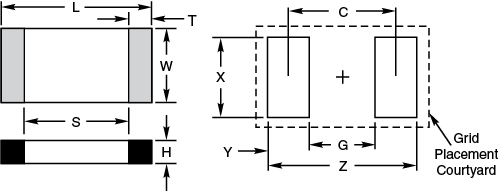
\includegraphics[width=.8\linewidth]{Figures/0402_landgrid} 
	\captionsource{The prototype connection}{Aurthor}
	\label{fig:sys_dia} 
\end{figure} 

Some of the design aspects used are described earlier and here they will be described in more detail.  
The industry standard is always good to aim for, in this case, the basic designs are taken from \gls{ipcg}'s design guidline\cite{ipcg}. While these are made for optimal manufacturability the footprints used on the test board are modified to enable for easier solderability, production and rework if needed. The landgrids are made slightly bigger and longer to achieve this. The downside of making the pads larger is that each component takes up more real estate and the final board size increases.

\subsection{Easy prototyping}
The components that are going to be used in high frequency often come in tiny packages. The best components used in this area of work will be small to fit in small modern advanced systems like mobilephones and.  This gives the protypability problems with easy ability to solder and use, To make a

\section{Structure}
The product is constructed with a number of components, which all have a central role in the final product. They can all be seen in \autoref{fig:sys_dia}. A list of the major components and their function can be seen below:

\begin{itemize}[noitemsep] 
\item \gls{mcu}: The central part of an integrated system, handles all the calculations and the program code.
\item Radio: All the communications with the rest of the world will be handled by the radio, sending on the VHF and UHF band.
\item \gls{imu}: Movement detection is measured with an accelerometer, this to determine if the unit is in motion or lying still. 
\item \gls{ldo}: A Low-dropout regulator can supply the system with a smoother voltage because no switching is taking place.
\item Hall sensor: The hall sensor is used as a switch for the system by sensing if a magnet is nearby and then turning off the circuit.
\item \gls{rtc}: A real-time clock is important to acquire data at a specific set time. It is important that the clock is exact over the whole life of the product.
\end{itemize} 


\begin{figure}[H] 
	\centering 
	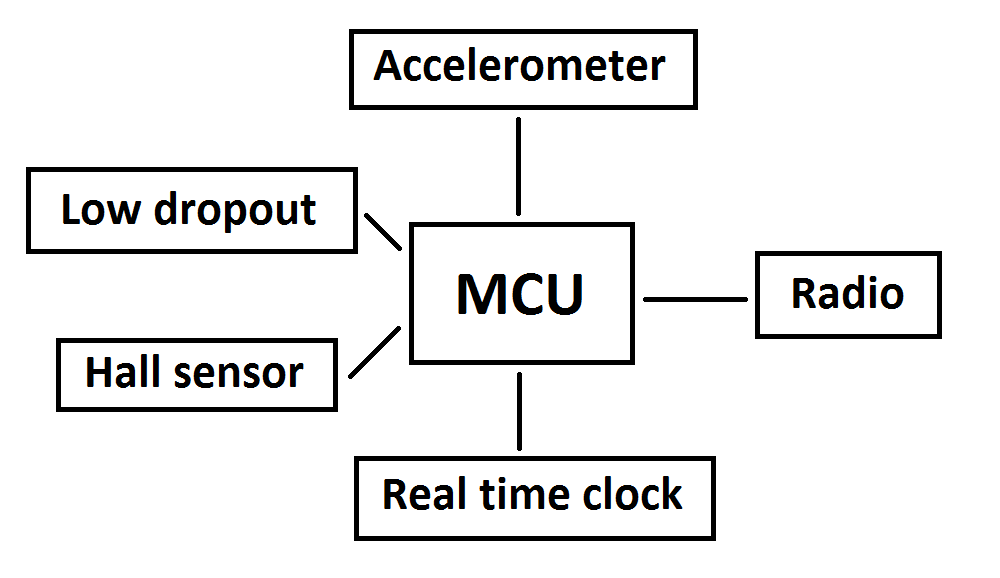
\includegraphics[width=.8\linewidth]{Figures/System_diagram} 
	\captionsource{The prototype connection}{Aurthor}
	\label{fig:sys_dia} 
\end{figure} 

Each of the components of this project is carefully chosen to get the functionality and effect that the company is after. To ensure the system works as intended the company has acquired development boards to each of the components. Every component needs to be tested to ensure their individual functionality. Each development board is connected to the microcontrollers board. First off, the \gls{mcu} have to be set up in a correct way with all its parameters and then the other components could be connected and initialized one after another. The whole connection can be seen. %\autoref{rattbo}.

%\begin{figure}[H] 
%\centering 
%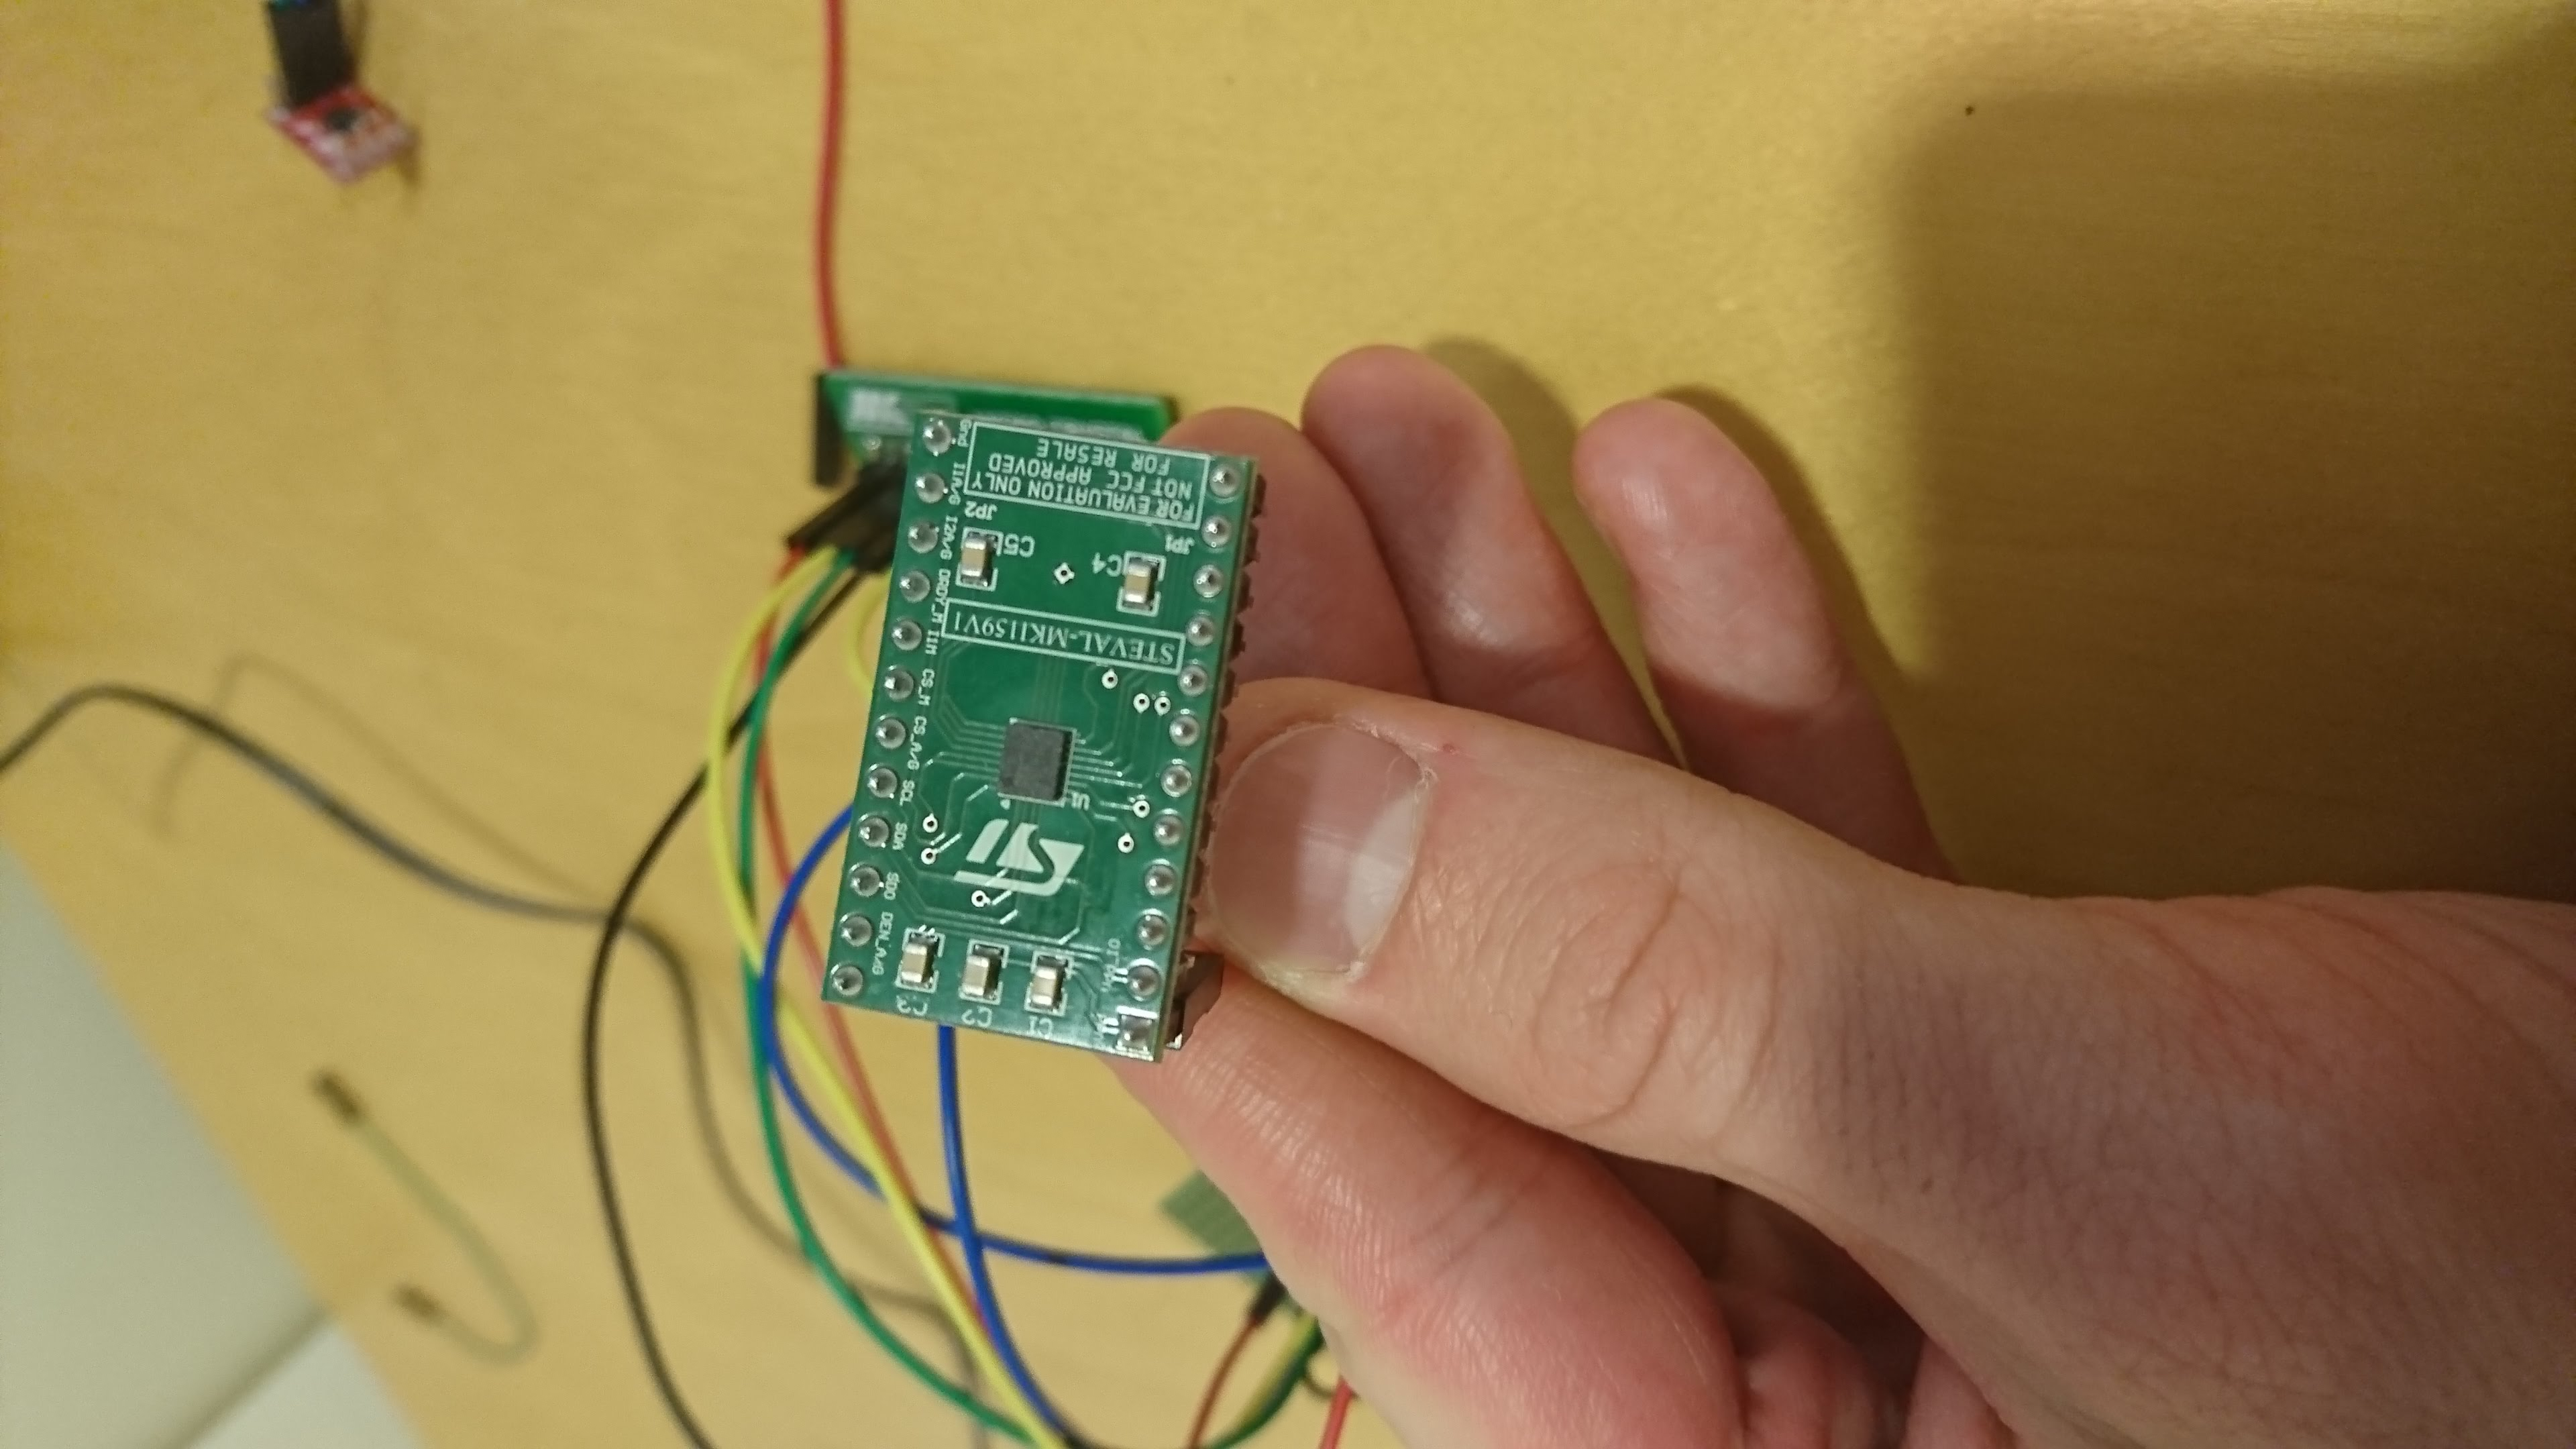
\includegraphics[width=.8\linewidth]{Figures/DSC_0103} 
%\captionsource{The prototype connection}{\url{Aurthor}}
%\label{rattbo} 
%\end{figure} 

%The \gls{mcu} can dtad


\section{Micro Controller Unit}
Every advanced system needs a central processing unit to make all the calculations needed. Why a lot of systems needs some powerful processor this system wich is a bit easier with 
The power consumption is higly dependent on the speed of which the processor is runnig, the faster the more power it consumes and also the slower the less current it will draw. And by the \gls{mcu} beeing the component with the single higest power consumption the speed is set to a speed as low as possible. This low speed is not a concern in this particular system when the operations required is not time or speed sensitive. The voltage supplied to the \gls{mcu} is another parameter that will alter the power consumption. The comonent is a low power model which can handle a lower source voltage. A voltage between 1.7 to 3.6 is required, anything lower will not start the device and anything higer will damage the the part. 
To get the right speed of a crystal we need to get the right product for this particular case. 
%As a crystal 
Many different types of oscillators exists, both internal and external types. 
The \gls{mcu} used for this project is a processor type that is used by this company many times before and has been chosen to this project for its small size, low power draw, sufficient connections, and features. The particular processor used is the PIC18LF46K22\cite{pic18}. The version used is one with 40 pins. All the connections available are shown in \autoref{Pic18_Pinout}.

\begin{figure}[H] 
\centering 
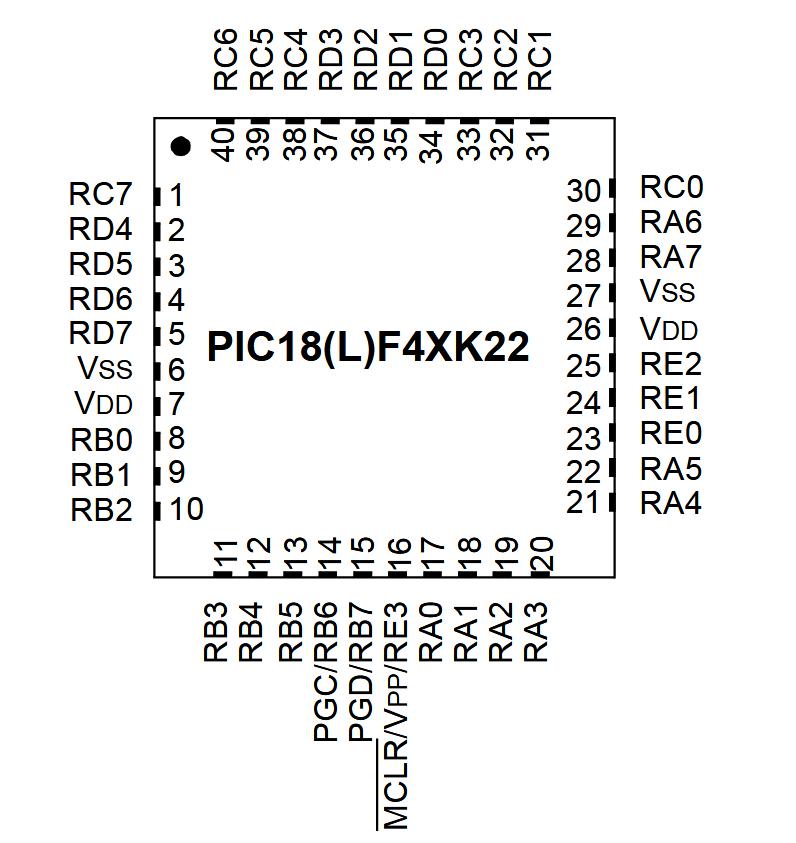
\includegraphics[width=.7\linewidth]{Figures/Pic18_pinout} 
\captionsource{PIC18LF46K22 pinout}{\url{http://ww1.microchip.com/downloads/en/DeviceDoc/40001412G.pdf}}
\label{Pic18_Pinout} 
\end{figure} 


%\subsection{Connenctions}

\subsection{Power}
Powering it is done by connecting the VDD pins to the power net. Connected to the ground is the Vss pins on the processor. To ensure the current fed is as smooth as possible capacitors are connected between these two pins. The value of these capacitors is chosen to 100nF.  

\subsection{Oscillator}
To operate the \gls{mcu} a clock signal is mandatory, this can be implemented in different ways. Either with the internal High, Medium and Low-frequency oscillator or an external one. Where the external rely on a specific circuitry to provide the clock source. Examples of external oscillators are clock modules, quartz crystal resonators or ceramic resonators and resistor-capacitor circuits. When a circuit is specified to be power efficient the speed of the clock plays a central role. As this product is specified to run on a small battery the speed of the system is kept low to increase the lifetime of the battery. The clock signal is generated from an external \gls{tcxo}.


\newpage %% Accelerometers
\section{Accelerometer} 
The motions of the system are measured with an \gls{imu} system. This system can be used in a lot of different cases, both to detect if the unit is stationary or moving or if there are very hard and fast movements in the product. One of the simplest \gls{imu}'s is the 3-axis accelerometer, it detects accelerations in three axes, x, y, and z. The component used is a 3-axis, ultra-low-power and high-performance accelerometer from \gls{st} \cite{ST_acc}. The component is the simplest of \gls{imu}'s that this manufacturer has and this simplicity makes for a product that is only incorporate one single function. 3-axis accelerometer means that it can measure  

\subsection{Connenctions}
Two voltage connections are apparent on this device, one which is called VDD and the other is called VDD-IO. The VDD is the supply voltage and VDD-IO determines the logic voltage level. 
No special attention is needed towards these contacts, both of them are connected to supply voltage. 

The component is connected to the MCU through the SPI interface, four wires are needed here. 

\newpage %% RTC
\section{Real Time Clock} 
Sending schemes with timed The \gls{rtc} is used to 

\subsection{Connenctions}
The component used in this project communicates with the \gls{i2c} interface, this requires two connections to the \gls{mcu}.


\newpage
\section{Radio component}
 The radio module used in this project is from the company Silabs. The chosen radio \gls{ic} have the characteristics that are wanted in this type of product. The radio transmission used is the earlier explained class E. With this pice the class E is already implemented in the radio as this is widely used today and a very effective radio signal. 
The type of filter used for sending radio signals at \gls{vhf} frequencies is defined in the defined 


\subsection{Connenctions}
 In the registers 


\newpage
\subsection{Solidworks PCB}
Followit uses the \gls{pcb} board design software Solidworks \gls{pcb} from DASSAULT SYSTÈMES. It utilizes the industry-proven Altium design engine for layout and routing of printed circuit boards and combined with a close connection with the mechanical \gls{cad} of classical Solidworks. With this program, the \gls{pcb} layout and design can be transferred seamlessly over to the mechanical environment to create an exact case or enclosure for the circuit board. The version used in this thesis is (Update 2.0).


\section{Power consumption}
 The total power consumption is calculated by adding the current draw from each individual component together.  A different test is conducted to try different modes of the system. One describing the power consumption of only the processor. This is done by running it in an infinite loop with all the other components at the circuit powered down or in power down mode. Since the system is not supposed to be active just a small time with a longer power down mode in between the power consumption on the system has to account for a longer time span. The tests are made with a standard scheme used already by the company. The scheme consists of a small radio pulse every second and the system being inactive in between these radio pulses. 
%All the systems 


%% 			Software
\clearpage
\chapter{Software}\label{sec:software}
\vspace{-10ex}%
\rule{\textwidth}{0.3pt}
\vspace{5ex}
 % after-code

%Method Software
\textit{
What is the step after the \gls{pcb} is produced? Yes it is time to test the system, and this is done with the help of a test program. This chapter will guide the reader through this process of setting up the processor to run program code. How all the components are programmed and tested will be explained in this chapter. 
}

%% MCU
\section{Programming} 
In start of every embedded system the processor have to be programmed. Here the most common implementation is the \gls{jtag}, where the all the programming and debugging is done through a standardized interface. The approach is different on this \gls{mcu}, here three pins are used to program the device. The first one is the "PGC", which is the clock signal for the In-Circuit Debugger and "PGD", In-Circuit Serial Programming. The third pin needed from the processor is the MCLR. These pins on the processor have to be accessible to program the microcontroller. %(Designing_Embedded_Systems_with_PIC_Microcontrollers 7.4.2)


\section{Software implementation}
The processor do not start up on it own, much consideration needs in making right initzilation and configure it right. A source voltage is supplied to the processor to get it to operate. There are some initial registers that needs to be set in order to inintialize and start the processor. This varies between different processors and models and is different for applications and systems. These registers contain information about the speed of the processor.    


\section{Radio implementation} %% Radio
Radio Chip Waking Up First,  the  radio  is  in  the  off  state. After  the  SDN  pin  is  pulled  low,  the  radio  wakes  up  and  performs  a  Power  on.
Reset  which  takes  a  maximum  of  6 ms  (900 $\mu$ s  typical  at  room  temperature)  until  the  chip  is  ready  to  receive commands on the SPI bus. The GPIO1 pin goes high when the radio is ready for receiving SPI commands. During the reset period, the radio cannot accept any SPI commands. 

\section{Software}
The fundation for every developmet is a good development enviroment, both as the circuit boards are createt and the software inplementations needed later in the process.

(In the early days of computing, programming in Assembler was used to program almost any type of
computer. These days, however, it is pretty much the preserve of embedded designers, particularly when
using smaller 8-bit devices) (PICDESIGN)

\subsection{MPLAB}
Microship which is the producer of the MCU used in this project have their own development enviroement with holds a lot of handy features when making a program for their products. 




\subsection{Assembly}
The acctual code that runs on this processor is assembly, the most common hardware code which is used in almost all types of MicroController units. Assembly is a harware type language which means that is describes the acctual process for the 

\subsection{C18}
The C program is compiled with the compiler C18. This is the compiler which have been the official compiler for this particular processor. This compiler is used for all the processors in the family PIC18. This complier is some years old and lacks some modern features. The vesion used in this project is (3.47)?

%% 			Results
\clearpage
\chapter{Results}\label{sec:results}
\vspace{-10ex}%
\rule{\textwidth}{0.3pt}
\vspace{10ex}

\emph{
This chapter will guide the reader through the whole process of developing a system prototype. Designing the PCB, soldering the components, troubleshooting the board and writing the necessary code are some of the steps involved and they will all be described in detail here.
}

\section{Schematics}
The schematics over the circuit is created by placing all the components discussed earlier, every IC have a small number of components that are placed in a way so that it is easy to understand which components belong to which. A title is added to every part in the design for a good overview of the system. Since the section which included the radio is large it is placed on a separate page. When additional components are added in additional pages can be inserted. These schematics can be found in \autoref{appendix_schematics}.

\section{Layout} 
\subsection{First design} The first of two boards is 3.5 times 3.5 mm in size. The different parts of the circuit are laid out in a way that it is easy to inspect and resolder if necessary. The main components of the board are placed close to each other at one side to get an idea of the design for the final product. This board is equipped with some test points for easy connections with test probes and oscilloscope. The silkscreen print on the top of the board was vague at some places and made distinguish them from each other hard. The pin one location at one part could not be spotted.  A view of the board can be seen in \autoref{PCB_rev1}. 

\begin{figure}[H]
	\centering
    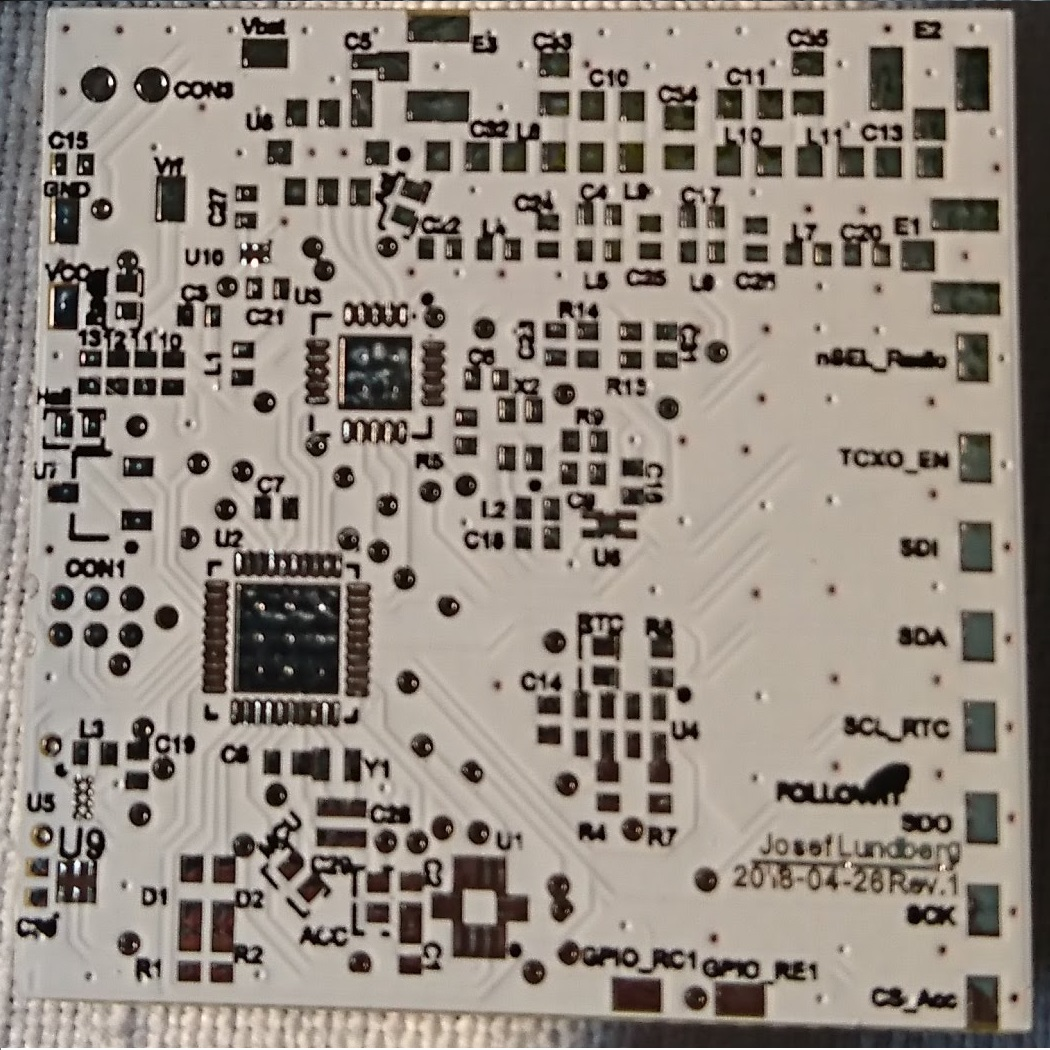
\includegraphics[width=.8\linewidth]{Figures/PWB}
	\captionsource{First (1) revision circuit board.}{Author}
	\label{fig:pcbr1}
\end{figure}

\section{Communication}

\subsection{UART}
The \gls{uart} connection interfered with another connection which leads to one function not working as intended. The function that is the enabling line to the \gls{ldo} which powers the oscillator for the radio. It is fixed by connection one of the extra pins that was laid out beforehand directly to the \gls{ldo}. The transmitting half of the \gls{uart} connection is working as intended on this version, some of the resulting data which is sent to the computer can be seen in \autoref{fig:uart_first_rev}.

\begin{figure}[H] 
    \centering 
    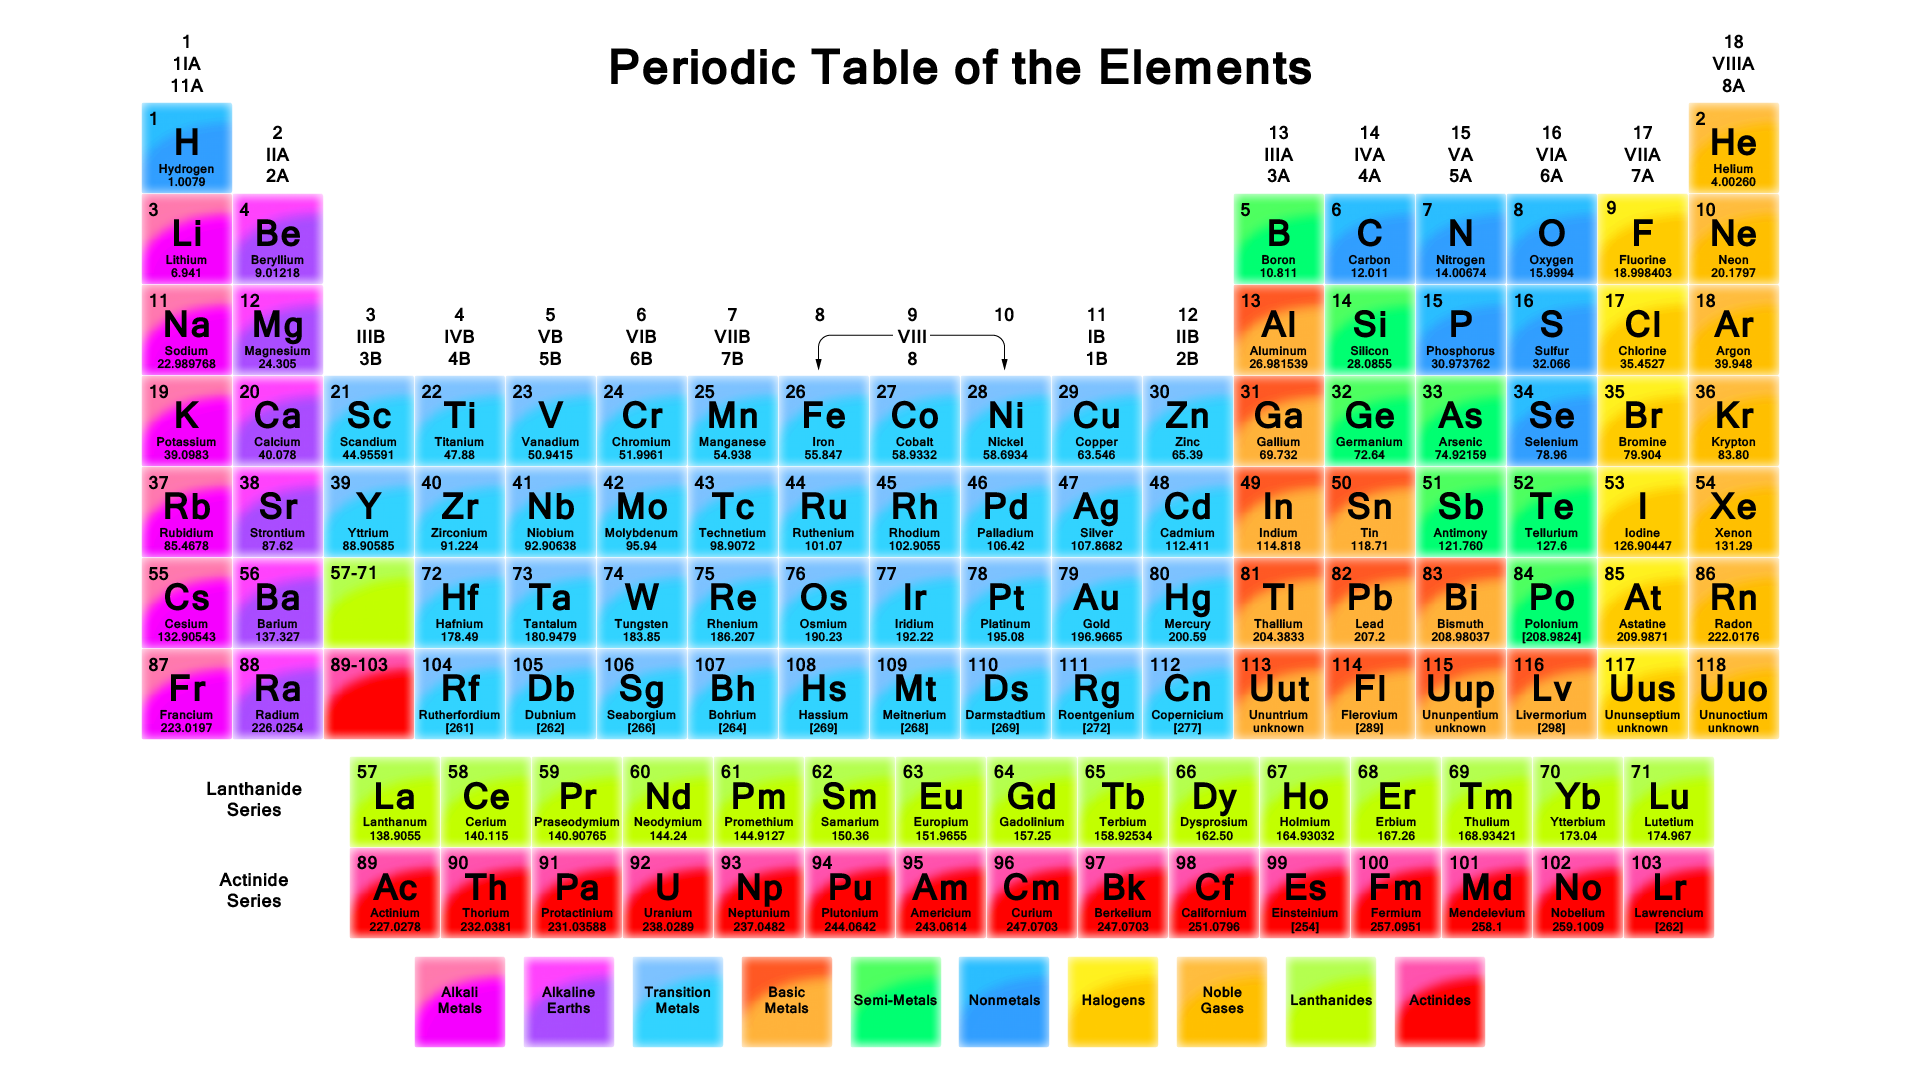
\includegraphics[width=.8\linewidth]{Figures/uart_first_rev} 
    \captionsource{Simple \gls{uart} transmission to a \gls{pc}}{Aurthor}
    \label{fig:uart_first_rev} 
\end{figure} 

\subsection{SPI}
Testing started with both the\gls{mcu}, radio and accelerometer soldered to the board. No communications were achieved when both of these slave devices were connected at the same time. After some troubleshooting, the failing factor of this is the accelerometer having it's \gls{spi} connection the other way around. The data out (SDO) line was connected to the data output, and the SDI was connected to the data input line of the accelerometer.  


\section{improvements}
From the first version some valuable point can be determined, both for the layout, schematics, and wiring.









% Kanske inte
\begin{comment}
\section{Power consumption}
When running the processor at operation speed and voltage the 
The power consumption is first mesured with only the processor connected. 
\end{comment}

%%			Schematics
\clearpage
\chapter{Schematics}\label{sec:schematic}
To the \gls{pcb} a schematic over the complete system has to be constructed. This is built by noting all the connections that were determined in earlier chapter.

%% 			Discussion
\clearpage
\chapter{Discussion}\label{sec:discussion}
The prototype could have been made directly using a company to place all the components, or the components should have been mounted with a pic and place machine to eliminate some initial troubleshooting and hassle regarding the SMT process. But with one of the projects goals to keep to expences down the process looked like this. This did however increase the understanding and personal expertice in the area. 

The test points were a good addition, they was frequently used and eployes at the company did found them intresting for furter use in future projects.
Additional test points whould be a good idea. When the board already had real estate to hold some additional points it should have been inplemented. 

The hardest bit with the system were the voltage adjusting buck converter. Both the fact that it was one of the smallest pieces and also the fact that it needed some adjustments in form of 

Designing a PCB with white soldermask looks great and with black silcskreen it was easy to see every marking. Problems did occur though, when visually inspecting the traces on the PCB it was hard almost inpossible to see. There is a reason that green is the most common choise. (The final design was therefore created with green soldermask)

To ease trobleshooting more a via could be placed in every single transmission line, this to be able to read the voltage levels and data at every trace. When building the first revision only some of the traces.

%% 			References
\clearpage
\begin{thebibliography}{99}
\label{sec:ref}
\addcontentsline{toc}{section}{\nameref{sec:ref}}

%%% BLANK LINKS

\bibitem{pic18}
	\url{http://ww1.microchip.com/downloads/en/DeviceDoc/40001412G.pdf}
\bibitem{STacc}
	\url{http://www.st.com/content/ccc/resource/technical/document/datasheet/group3/30/3a/4e/6b/68/16/4a/35/DM00323179/files/DM00323179.pdf/jcr:content/translations/en.DM00323179.pdf}

\begin{comment}
%% RFEWF

\bibitem{cad}
	\url{https://www.autodesk.com/products/fusion-360/overview}
\bibitem{wind_meas}
	\url{ltu.diva-portal.org/smash/get/diva2:1039147/FULLTEXT01.pdf}
\bibitem{load_cell}
	\url{http://www.te.com/commerce/DocumentDelivery/DDEController?Action=srchrtrv&DocNm=FX19&DocType=DS&DocLang=English}
\bibitem{webpage}
	\url{http://www.lygte-info.dk/info/battery\%20protection\%20UK.html}


%%% LINKS WITH DESCRIPTIONS
\bibitem{lm1117}
	KiCad library entry for voltage regulator component lm1117 by \emph{ObKo}, 2012,
	\url{https://github.com/ObKo/kicad-libraries/blob/master/libraries/lm1117.lib}.
\bibitem{overprotection}
	Overvoltage and Reverce-voltage Protection in Automotive Systems,
	Application note 760, \emph{Maxim integrated}, Apr 02, 2002, 
	\url{https://www.maximintegrated.com/en/app-notes/index.mvp/id/760}.
\bibitem{Tof_cover}
	\gls{st}, Application note: AN4907, \emph{VL53L0X ranging module cover window guidelines},
	\url{http://www.st.com/content/ccc/resource/technical/document/application_note/group0/9d/93/be/33/13/be/46/19/DM00326504/files/DM00326504.pdf/jcr:content/translations/en.DM00326504.pdf}
\bibitem{kf eff}
	Duygun, M., Kutlu, L. \& Sickles, R.C., Journal of Productivity Analysis, 2016, 46: 155, \url{https://doi.org/10.1007/s11123-016-0477-z}
%%% NO LINK STUFF
\bibitem{cccv}
	Power Guy, \emph{Constant Current Constant voltage}, May 26, 2016, San Diego, USA,
	\url{https://www.us.tdk-lambda.com/media/292143/tdk-lambda-blog-052616.pdf}.
\bibitem{animal} 
	D.L. Hall and J. Llinas, \emph{An introduction to multisensor data fusion}, 
	Proceedings of the IEEE, 85(1):6 –23, jan 1997.
\bibitem{boken} 
	B.R. Grover H, Patrick, \emph{Introduction to random signals and applied Kalman filtering}, 1997. 
\bibitem{SNAME} 
	Society of Naval Architects and Marine Engineers (SNAME), \emph{Principles of Naval Architecture}, 1989, Vol. III, \emph{SNAME}. 
\bibitem{nonlinear} 
	Dr. Oliver Nelles, \texttt{nonlinear system identification}.
\bibitem{non-linear}
	Noureldin., Karamat T.B., Georgy J., 2013, \texttt{ Basic Navigational Mathematics, Reference Frames and the Earth’s Geometry. In: Fundamentals of Inertial Navigation, Satellite-based 	Positioning and their Integration}, Springer, Berlin, Heidelberg.
\bibitem{animal}
	D.L. Hall and J. Llinas. \emph{An introduction to multisensor data fusion}, Proceedings of the. IEEE, 85(1):6 –23, jan 1997.
\bibitem{signal_process}
	Henry Stark, John W Woods, \emph{Probability and Random Processes with Applications to Signal Processing}, 4/E 2012,
	 Pearson Higher Education.
\bibitem{Discrete_kalman}
	Donald E. Catlin, \emph{Estimation, Control, and the Discrete Kalman Filter}, 1989.
\bibitem{book}
	Weicker, P., \emph{A Systems Approach to Lithium-ion Battery Management}, Boston, Artech House, 2014.
\end{comment}
\end{thebibliography}


%%			Appendix
\clearpage
\begin{appendices}
\section{Large Figures}\label{sec:app}

\clearpage
\section{Lists}
\subsection{Bill of Materials: Main \gls{pcb}}
\begin{center}
\begin{tabular}{|l|l|c|}
	\hline
	\bf{Main Board Components} & \bf{Package} & \bf{Quantity} \\
	\hline
	\emph{Capacitors:} & & \\
	\hline
	18p & 0805 & 2 \\
	\hline
	100n & 0805 & 21 \\
	\hline
	1u & 0805 & 2 \\
	\hline 
	2.2u & 0805 & 1 \\
	\hline 
	4.7u & 0805 & 4 \\
	\hline 
	10u & Electrolytic SMD 5x5.3 & 6 \\
	\hline
	\emph{Resistors:} & & \\
	\hline
	220 & 0805 & 1 \\
	\hline
	1k & 0805 & 2 \\
	\hline
	1k & potentiometer & 2 \\
	\hline

\end{tabular}
\end{center}

\clearpage
\subsection{Bill of Materials: Battery Management \gls{pcb}}
%\begin{center}
\begin{tabular}{|l|l|c|}
	\hline
	\bf{Battery Management Circuit} & \bf{Package} & \bf{Quantity} \\

	30.1k & 0603 & 1 \\
	\hline
	32.4k & 0603 & 2 \\
	Power P-MOS & SOT-23 & 1 \\
	\hline
\end{tabular}
%\end{center}
%Image of circuit board(s) are sectionlocals labled as "fig:pcbr*"
%Local. Image of casing
%INSERT Image of complete/mounted system
\end{appendices}

\newpage
\vspace*{9cm}
\begin{center}
The project; complete with all software code, the application, hardware files and more, can be found online in the github-repo:\\
\url{https://github.com/Jurriz/VHF-Unit}
\end{center}

\end{document}
